\chapter{Geometría}

\section{Trigonometría}
\begin{align*}
\sin(\alpha \pm \beta)&{}=\sin \alpha \cos \beta \pm \cos \alpha \sin \beta\\
\cos(\alpha \pm \beta)&{}=\cos \alpha \cos \beta \mp \sin \alpha \sin \beta\\
\tan(\alpha \pm \beta)&{}=\dfrac{\tan \alpha \pm \tan \beta}{1 \mp \tan \alpha \tan \beta}\\
\sin \alpha + \sin \beta &{} = 2\sin\dfrac{\alpha + \beta}{2}\cos\dfrac{\alpha - \beta}{2}\\
\cos \alpha + \cos \beta&{}=2\cos\dfrac{\alpha + \beta}{2}\cos\dfrac{\alpha - \beta}{2}
\end{align*}


%\[ (V+W)\tan(v-w)/2{}=(V-W)\tan(v+w)/2 \]
%where $V, W$ are lengths of sides opposite angles $v, w$.
%\begin{align*}
%a\cos x+b\sin x&=r\cos(x-\phi)\\
%a\sin x+b\cos x&=r\sin(x+\phi)
%\end{align*}
%where $r=\sqrt{a^2+b^2}, \phi=\operatorname{atan2}(b,a)$.


\section{Triángulos}
En un triángulo de lados $a,b,c$, alturas $h_a, h_b, h_c$, medianas $m_a, m_b, m_c$, semiperímetro $s = \dfrac{a + b + c}{2}$ y área $A$.\\
\medskip

\begin{description}
	\item[Heron-like area formulae]
		\begin{align*} 
		A &= \sqrt{s(s-a)(s-b)(s-c)}\\
			% UVa 10522, https://www.cambridge.org/core/journals/mathematical-gazette/article/8980-a-heron-type-formula-for-the-reciprocal-area-of-a-triangle/7570E2DA337B8A6339CB4DA3356204F4
			&= \left( 4 \sqrt{\eta (\eta - h_a^{-1}) (\eta - h_b^{-1}) (\eta - h_c^{-1})} \right)^{-1} \\
			% UVa 10347, https://math.stackexchange.com/questions/396085/how-to-find-area-of-triangle-from-its-medians/923165#923165
			&= \dfrac{4}{3} \sqrt{s(s - m_a)(s - m_b)(s - m_c)}
		\end{align*}
		
		donde $\eta = \dfrac{1}{2} (h_a^{-1} + h_b^{-1} + h_c^{-1})$
	\item[Circunradio] $R = \dfrac{abc}{4A}$
	\item[Inradio] $r=\dfrac{A}{s}$
	\item[Medianas] dividen en dos subtriángulos de igual área. %https://es.wikipedia.org/wiki/Teorema_de_Apolonio
		\begin{equation}
			\tag{teorema de Apolonio}
			m_a=\dfrac{1}{2}\sqrt{2b^2 + 2c^2 - a^2}
		\end{equation}
	\item[Bisectrices] dividen a los ángulos en dos partes iguales.
		\[ b_a=\sqrt{bc\left(1-\left(\dfrac{a}{b+c}\right)^2\right)}\]
	\item[Teorema del seno]
	$ \dfrac{\sin\alpha}{a}=\dfrac{\sin\beta}{b}=\dfrac{\sin\gamma}{c}=\dfrac{1}{2R}$
	\item[Teorema del coseno]
	$ a^2=b^2+c^2-2bc\cos\alpha $
	\item[Teorema de la tangente]
	$ \dfrac{a+b}{a-b}=\dfrac{\tan\dfrac{\alpha+\beta}{2}}{\tan\dfrac{\alpha-\beta}{2}} $
\end{description}

\section{Cuadriláteros}

	\subsection{Cuadriláteros cíclicos}
	Sea un cuadrilátero \textbf{cíclico} de lados $a, b, c, d$ y diagonales $e, f$. Entonces $ef = ac + bd$ y el área $A$ se puede calcular con la
	
	\begin{description}
		\item[Fórmula de Brahmagupta]
		\[A = \sqrt{(s - a)(s - b)(s - c)(s - d)}\]
		donde $s = \dfrac{a + b + c + d}{2}$
	\end{description}

\section{Coordenadas esféricas}
	\centerline{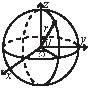
\includegraphics[width=25mm]{../content/matematicas/sphericalCoordinates}}
	\[\begin{array}{cc}
	x = r\sin\theta\cos\phi & r = \sqrt{x^2+y^2+z^2}\\
	y = r\sin\theta\sin\phi & \theta = \texttt{acos}(z/\sqrt{x^2+y^2+z^2})\\
	z = r\cos\theta & \phi = \texttt{atan2}(y,x)
	\end{array}\]

\section{Puntos y vectores}
	\chuletarioimport{Point.h}{{12-35}}%
		[\texttt{struct} para representar puntos y vectores en el plano. \texttt{T} puede ser \texttt{double} o \texttt{ll}, por ejemplo (por lo general evita \texttt{int}). Si usas enteros, asegúrate de que aunque los datos te los den en coordenadas enteras, todos los cálculos que hagas con ellos también.]
		
	\chuletarioimport{pointVec.cpp}{}%
		[\texttt{struct}s para representar puntos y vectores en el plano como en el Halim, con algunas operaciones básicas.]

\section{Rectas y segmentos}
	\chuletarioimport{lines.cpp}{}%
		[\texttt{struct} para representar rectas en el plano $ax + by + c = 0$, con algunas operaciones básicas.]
		
	\chuletarioimport{lineIntersect.cpp}{}%
		[Devuelve \texttt{true} si las rectas \texttt{l1} y \texttt{l2} no son paralelas, y en tal caso devuelve en \texttt{p} el punto de intersección.]
		
	% UVa 273
	% Basado en https://stackoverflow.com/questions/563198/how-do-you-detect-where-two-line-segments-intersect
	\chuletarioimport{segmentIntersect.cpp}{}%
		[Devuelve \texttt{true} si los segmentos \texttt{a} y \texttt{b} intersecan.\\
		Si los segmentos intersecan, devuelve en \texttt{x} un punto de intersección.\\
		Si los segmentos intersecan, devuelve en \texttt{collinear} si los segmentos son colineales. Si lo son, hay o bien un único punto de intersección (los segmentos se tocan en un extremo), o infinitos (los segmentos se solapan). Si no son colineales, el punto de intersección es único.\\
		Un segmento está representado por $p + \lambda \vec{r}, \lambda \in [0, 1]$.]

	\chuletarioimport{distToLine.cpp}{11-17}%
		[Devuelve la distancia desde \texttt{p} a la línea que pasa por los puntos \textbf{distintos} \texttt{a} y \texttt{b}. El punto más cercano a \texttt{p} sobre la línea se guarda en \texttt{c}.]
	
	\chuletarioimport{distToSegment.cpp}{11-22}%
		[Devuelve la distancia desde \texttt{p} al segmento que pasa por los puntos \textbf{distintos} \texttt{a} y \texttt{b}. El punto más cercano a \texttt{p} sobre el segmento se guarda en \texttt{c}.]

\section{Círculos}

	\chuletarioimport{Circles.cpp}{}%
		[Construcción de círculos notables: con dos puntos y el radio, circunferencias circunscrita e inscrita. A veces se necesitará el área: usa la fórmula de Herón.]
	
	\chuletarioimport{tangentPoints.cpp}{}% UVa 10180
		[Dado un punto \texttt{p}, fuera del círculo $x^2 + y^2 = r^2$, devuelve en el array \texttt{pt} los dos puntos de tangencia de las rectas tangentes al círculo desde \texttt{p}.]
		
	\chuletarioimport{circle3pts.cpp}{}%
		[Dados tres puntos no alineados, devuelve el centro del único círculo que pasa por esos tres puntos.] % TODO: https://math.stackexchange.com/questions/213658/get-the-equation-of-a-circle-when-given-3-points

\section{Polígonos}
	\begin{description}
		\item[Teorema de Pick] Sea un polígono simple cuyos vértices tienen coordenadas enteras. Si $B$ es el número de puntos enteros en el borde, $I$ el número de puntos enteros en el interior del polígono, entonces el área $A = I + \dfrac{B}{2} - 1$.
	\end{description}

	En lo que sigue, representamos un polígono por un vector de puntos dados en sentido antihorario en el que el primer punto y el último punto son el mismo (i.e. \texttt{P[0]} $=$ \texttt{P[n - 1]}).
	
	\chuletarioimport{areaPerimeter.cpp}{}%
		[Calcula el área y el perímetro del polígono \texttt{P}.]
	
	\chuletarioimport{inPolygon.cpp}{}%
		[Devuelve \texttt{true} si el punto \texttt{pt} está dentro del polígono \texttt{P}. ¿Qué pasa si \texttt{pt} está sobre una arista del polígono?]%
		[][\bigo{n}]
		
	\chuletarioimport{inConvexPolygon.cpp}{}%
		[Devuelve \texttt{true} si el punto \texttt{q} está en dentro del polígono \textbf{convexo} (dado en sentido antihorario).]%
		[][\bigo{\log n}]

	\chuletarioimport{cutPolygon.cpp}{}%
		[Corta el polígono \texttt{Q} con la recta dada por los puntos \texttt{a} y \texttt{b}. Devuelve la parte izquierda del corte (\texttt{a} y \texttt{b} formarán parte del polígono a devolver).\\
		Para hacer la programación más simple se hace uso de \texttt{lineIntersectSeg}, que interseca un segmento con una recta.]%
	
	\chuletarioimport{grahamScan.cpp}{}%
		[Calcula la envolvente convexa de una nube de puntos.\\
		 No da el resultado correcto si \texttt{P} son tres puntos alineados.\\
		 Da excepción en ejecución si \texttt{P} empieza con cuatro puntos alineados.\\
		 Precisa de \texttt{angleCmp} para ordenar los puntos según el ángulo que formen con el eje $x$.]%
		 [][\bigo{n \log n}]	
	% https://en.wikibooks.org/wiki/Algorithm_Implementation/Geometry/Convex_hull/Monotone_chain
	\chuletarioimport{andrewsMonotoneChain.cpp}{}%
		[Devuelve un polígono con la envolvente convexa de una nube de puntos.]%
		[][\bigo{n \log n}]

\section{Misc.}

TODO: Apotema, teorema de stewart, volúmenes de pirámides, cone frustums...

% Adaptado de https://github.com/radoslav11/Coding-Library/blob/master/geometry/closest_points.cp
% Explicado en el Cormen
\chuletarioimport{closestPoints.cpp}{}%
	[Devuelve la closest pair distance de una nube de puntos. Esquema útil para algoritmos de divide y vencerás.]%
	[][\bigo{n \log n}]

\subsection{Great Circle distance}
	\chuletarioimport{sphericalDistance.cpp}{}%

	\chuletarioimport{SphericalDistance.cpp}{}%
		[Calcula la distancia entre 2 puntos sobre una esfera dados sus ángulos $\phi$ y $\theta$ y el radio de la esfera. Para ello, pasa primero a cartesianas.]